\documentclass{standalone}
\usepackage[usenames,dvipsnames]{xcolor}
\usepackage{tikz}
\usepackage{amssymb, amsmath}
\usetikzlibrary{calc, intersections, arrows, backgrounds}

\begin{document}
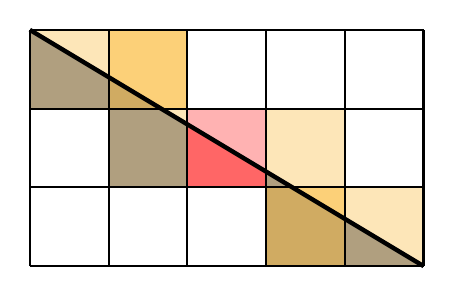
\begin{tikzpicture}
  \draw[thick] (0, 0) grid (5, 3);
  \draw[ultra thick] (5, 0) -- (0, 3);
  \foreach \x/\y/\c in {0/2/30,1/2/60,1/1/30,3/1/30,3/0/60,4/0/30} {
  \begin{scope}[on background layer]
    \begin{scope}
    \path[clip] (0, 0) -- (5, 0) -- (0, 3) -- cycle ;
    \fill[Dandelion!\c!gray] (\x, \y) rectangle (\x+1, \y+1);
    \end{scope}
  \end{scope}
  \begin{scope}[on background layer]
    \begin{scope}
    \clip (5, 3) -- (0, 3) -- (5, 0) -- cycle;
    \fill[Dandelion!\c] (\x, \y) rectangle (\x+1, \y+1);
    \end{scope}
  \end{scope}
  }
  \begin{scope}[on background layer]
    \begin{scope}
    \path[clip] (0, 0) -- (5, 0) -- (0, 3) -- cycle ;
    \fill[red!60] (2,1) rectangle (3, 2);
    \end{scope}
    \begin{scope}
      \path[clip] (5, 3) -- (5, 0) -- (0, 3) -- cycle ;
      \fill[red!30] (2,1) rectangle (3, 2);
      \end{scope}
  \end{scope}
\end{tikzpicture}
\end{document}